\chapter{Patrones de Diseño}
\label{patrones}

\section{¿Qué son?}

En principio, se puede pensar a un patrón como una manera especialmente inteligente e intuitiva de resolver una clase de problema en particular. Según Christopher Alexander:

\begin{center}
\emph{``... un patrón describe un problema que sucede una y otra vez en nuestro entorno, y luego describe el núcleo de la solución a ese problema, de tal forma que puede utilizar esa solución un millón de veces más, sin siquiera hacerlo dos veces de la misma manera.''}
\end{center}

Los patrones de diseño\cite{Gamma95} existen independientemente de cualquier implementación particular y pueden implementarse de diversas maneras. Básicamente se clasifican según tres propósitos:
\begin{enumerate}
	\item \emph{Creacional:} tiene que ver del Cómo se puede crear un objeto. Habitualmente incluye aislar los detalles de la creación
							 del objeto, de forma que su código no dependa de los tipos de objeto que hay y por lo tanto, no es
							 necesario cambiarlo cuando se añade un nuevo tipo de objeto. Ejemplos: \emph{Singleton}, \emph{Abstract
							 Factory}, \emph{Factory Method}, entre otros.

	\item \emph{Estructural:} cuando afecta a la manera en que los objetos se conectan con otros objetos para asegurar que los cambios
							 del sistema no requieren cambiar esas conexiones. Ejemplos: \emph{Proxy}, Ejemplos: \emph{Adapter}, entre
							 otros.

	\item \emph{Comportamiento:} se emplean cuando los objetos manejan tipos particulares de acciones dentro de un programa. Éstos encapsulan procesos que quiere que se ejecuten, como interpretar un lenguaje, completar una petición, moverse a través de una secuencia  implementar un algoritmo. Ejemplos: \emph{iterator}, \emph{State}, \emph{Observer}, \emph{Strategy}, entre otros.
\end{enumerate}

\section{Patrones Empleados}

\subsection{Singleton}
\label{singleton}       
Corresponde al patrón de diseño más simple de todos, que se aplica cuando sólo se requiere una única instancia de una clase.

\begin{figure}[h!]
	\hspace*{3.5cm} 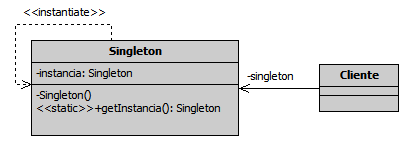
\includegraphics[scale=0.7]{image/singleton.png}
	\caption{Patrón Singleton [21].}	
\end{figure} 

\subsection{Factory Method}
\label{factoryMethod}
Consiste en definir una interface para crear objetos de tipo generico permitiendo a las subclases decidir que tipo de objetos concretos crear. Es similar al \emph{Abstract Factory} pero sin el énfasis en las familias. Es un patrón muy útil dado que permite escribir aplicaciones que son más flexibles respecto de los tipos a utilizar difiriendo la creación de las instancias en el sistema a subclases que pueden ser extendidas a medida que se extiende el sistema. 

\begin{figure}[h!]
	\hspace*{1cm}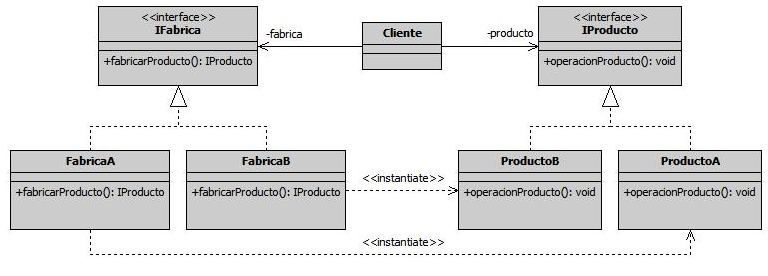
\includegraphics[scale=0.4]{image/factoryMethod.png}
	\caption{Patrón Factory Method [22].}	
\end{figure} 

\begin{verbatim}
struct Speaker
{
    virtual void saySomething() = 0;
    virtual ~Speaker(){}
};

class Hello: public Speaker
{
    virtual void saySomething();
};

void Hello::saySomething()
{
    std::cout << "Hello" << std::endl;
}

REGISTER_FACTORIZABLE_CLASS(Speaker, Hello, std::string, "Hello");

class Goodbye: public Speaker
{
    virtual void saySomething();
};

void Goodbye::saySomething()
{
    std::cout << "Goodbye" << std::endl;
}

REGISTER_FACTORIZABLE_CLASS(Speaker, Goodbye, std::string, "Goodbye");

int main()
{
	Speaker* speaker = mili::FactoryRegistry<Speaker, std::string>::new_class("Hello");
	speaker->saySomething();
	delete speaker;
	return 0;
}

Output: Hello
\end{verbatim}

\subsection{Observer}
\label{observer}
Define una dependencia del tipo $1->N$ entre objetos, de tal forma que cuando el objeto cambia de estado, todos sus objetos dependientes son notificados automáticamente. Los objetos observadores se añadan a una lista de objetos, y el objeto observado notificará el cambio a todos los objetos de esta lista cuando se produzca el cambio. Básicamente se aplica cuando se necesita consistencia entre clases relacionadas, pero con independecia, es decir, con un bajo acoplamiento. 

\begin{figure}[h!]
	\centering
		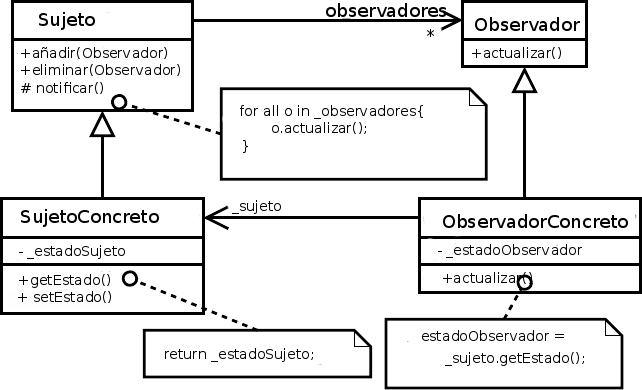
\includegraphics[scale=0.4]{image/observer.png}
	\caption{Patrón Observer [23].}
\end{figure} 	

Un funcionamiento básico de este patrón se exhibe en la figura ~\ref{observerDiagram}.

\begin{figure}[h!]
	\centering
		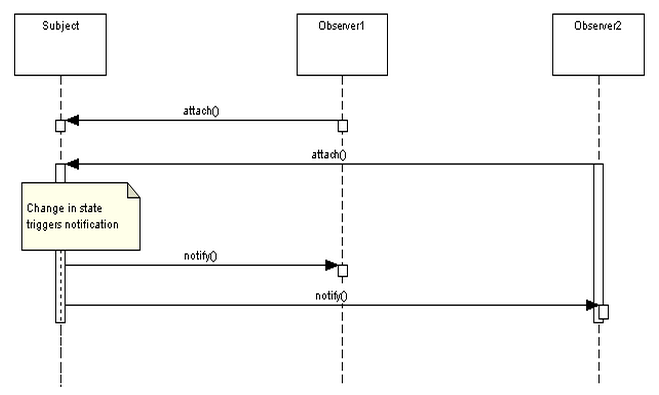
\includegraphics[scale=0.5]{image/observerDiagram.png}
	\caption{Diagrama de Secuencias Observer [24].}
	\label{observerDiagram} 
\end{figure}

\subsection{Template Method}
\label{templateMethod}

\par Corresponde a un patrón de diseño de comportamiento. Este tipo de patrón ayuda a resolver problemas de interacción entre clases y objetos. Surge de la necesidad de extender determinados comportamientos dentro de un mismo algoritmo por parte de diferentes entidades. Es decir, diferentes entidades tienen un comportamiento similar pero que difiere en determinados aspectos puntuales en función de la entidad concreta. Una posible solución consiste en copiar el algoritmo en cada de las diferentes entidades cambiando la parte concreta en la que difieren, aunque tiene una consecuencia negativa ya que se genera código duplicado.  
\par La solución que propone el mencionado patrón es abstraer todo el comportamiento que comparten las entidades en una clase (abstracta) de la que, posteriormente, extenderán dichas entidades. Esta superclase definirá un método que contendrá el esqueleto de ese algoritmo común (método plantilla) y delegará determinada responsabilidad en las clases hijas, mediante uno o varios métodos abstractos que deberán implementar. La estructura del patrón se exhibe en la figura~\ref{templateMethod}.

\begin{figure}[h!]
	\centering
		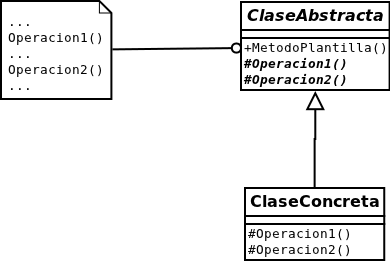
\includegraphics[scale=0.5]{image/templateMethod.png}
	\caption{Template Method [25].}
	\label{} 
\end{figure}

\par Es un patrón que se adecuada cuando contamos con un algoritmo con varios pasos que no cambian, de modo que dichos pasos invariantes serían implementados en una superclase, dejando la implementación de los pasos que cambian para las subclases. A continuación se muestra un ejemplo del patrón en pseudo-código:

\begin{lstlisting}[basicstyle=\tt, frame=trBL, tabsize=4,fontadjust=true]
class Base
{
  public:
    void execute()
    {
        a();
        ph1();
        c();
        ph2();
        e();
    }
  private:
    void a() { ... }
    void c() { ... }
    void e() { ... }    
    virtual void ph1() = 0;
    virtual void ph2() = 0;
};

class One: public Base
{
    /*virtual*/void ph1() { ... }
    /*virtual*/void ph2() { ... }    
};

class Two: public Base
{
 	/*virtual*/void ph1() { ... }
    /*virtual*/void ph2() { ... }       
};
	
\end{lstlisting}
\hspace*{2cm}\caption{Código D.1: Pseudo-código patrón Template Method.}

\subsection{Mediator}
\label{mediator}
\par El patrón de diseño \emph{Mediator} está considerado como un patrón de comportamiento. Básicamente encapsula la comunicación entre muchas clases mediante un objeto mediador.

\par En POO seguramente se tendrán que crear un montón de clases que interactúan entre sí. Si no se aplican ciertos principios, cada objeto dependerá de muchos otros. Con el fin de evitar marcos acoplados, surge el patrón mediador para facilitar la interacción entre los objetos de una manera en la que cada objeto no es conscientes de la existencia de otros objetos.

\par En la figura~\ref{mediador} se exhibe un ejemplo de uso presente patrón.

\begin{figure}[h!]
	\centering
		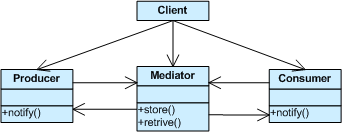
\includegraphics[scale=0.7]{image/mediador.png}
	\caption{Ejemplo patrón Mediator [18].}
	\label{mediador} 
\end{figure}
